\documentclass{article}

\usepackage{xcolor}
\usepackage{geometry}
\geometry{a4paper, total={170mm,257mm},left=20mm, top=20mm,}

\usepackage{pgf}
\usepackage{tikz}
\usetikzlibrary{arrows,automata}

\title{Évaluation d’expressions booléennes}
\author{LAZZARI-ARMOUR Raphael et POULIQUEN Chloé}
\date{Dimanche XX Mai 2021}

\begin{document}

\maketitle

\section*{Question 1}
\textit{
\textcolor{blue}{
\underline{Question:}
 Lire une chaîne de caractère contenant une expression arithmétique et la transformer en une liste de tokens.
}
}
\newline\newline
Pour cette première question, nous avons eu besoin de définir la structure suivante. Le but du projet étant sur les "expressions booléennes", nous avons décidé de faire une structure composé uniquement de booléen. La taille d'un booléen étant de 1 bit, cela nous fait par la même occasion économiser sur la mémoire allouée pour la liste par la suite. 

\begin{verbatim}
struct token{
  struct token* next;
  type TYPE;
  union{
    bool value;             //if TYPE is a CONSTANT, value is 'true' if '1' else 'false' if '0'
    bool bracket;           //if TYPE is a BRACKET, value is 'true' if '(' else 'false' if ')'
    bool unary;             //if TYPE is a UNARY_OP, value is 'true' if 'NON' else 'false'
    op_binary OpBinary;     //if TYPE is a BINARY_OP, value depends on enum op_binary
  }attribute;
};
typedef struct token* TokenList;
\end{verbatim}

L'appel de la fonction \textit{TokenList $string\_to\_token(char* string)$} dans le main nous permet de convertir la chaîne de caractère entrée par l'utilisateur en une liste de token. Cette fonction prends en paramètre une chaîne de caractères et retourne une liste de tokens. 

\section*{Question 2}
\textit{
\textcolor{blue}{
\underline{Question:} 
Donner un automate à pile reconnaissant le langage dont les mots sont les expressions
booléennes.
}
}
\newline\newline
Pour cette question, nous proposant un automate reconnaissant le langage par état final et par pile vide. 
Une pile qui empile '(' et dépile ')'.
\newline\newline
\underline{Règle sur les constantes '0' et '1':}
Doit contenir un opérateur binaire, unaire ou '(' avant mais pas une autre constante. Peut être suivi par un opérateur binaire ou ')' mais pas par une constante. 
\newline\newline
\underline{Règle sur les opérateurs binaires '+' , '.' , '$\Rightarrow$' et '$\Leftrightarrow$' :}
Doit contenir une constante ou ')' avant et doit contenir une constante ou '(' après. 
\newline\newline
\underline{Règle sur l'opérateur unaire 'NON' et '(':}
Ne peut pas contenir une constante avant. L'opérateur 'NON' doit être suivi par une constante ou par l'opérateur '('. Il ne peut ainsi pas être suivi par un opérateur binaire ou par ')'. 
\newline\newline
Après étude de ces règles, on peut définir l'automate suivant:
\newline
\newline 
On définit notre automate de la façon suivante:
\newline
\newline
\begin{math}
A = (\Sigma,\;Q,\;q_0,\;\Gamma,\delta,\;F,\;T)
\newline\newline
avec:\newline	
		\Sigma = \{NON \; ,\; ( \; , \; ) \; , \; 1 \; , \; 0 \; , \; \Leftrightarrow \; , \; + \; , \; . \; , \; \Rightarrow\}
	\newline
		Q = \{q_0 \; , \; q_1\}
	\newline
		q_0 = q_0
	\newline
		\Gamma = \{X\}
	\newline
		\delta = \delta
	\newline
		F = \{q_1\}
	\newline
		T = \{ \;\;	(q_0 \; , \; \delta \; , \; non \; , \; \delta   \; , \; q_0) \; , \;
				(q_0 \; , \; X 	    \; , \; non \; , \; X        \; , \; q_0) \; , \;
				(q_0 \; , \; \delta \; , \; (   \; , \; \delta X \; , \; q_0) \; , \;
				(q_0 \; , \; X      \; , \; (   \; , \; XX       \; , \; q_0) \newline
		\hspace*{1,1cm} (q_0 \; , \; \delta \; , \; 1   \; , \; \delta   \; , \; q_1) \; , \;
				(q_0 \; , \; X      \; , \; 1   \; , \; X        \; , \; q_1) \; , \;				
				(q_0 \; , \; \delta \; , \; 0   \; , \; \delta   \; , \; q_1)
\; , \; 
				(q_0 \; , \; X      \; , \; 0   \; , \; X        \; , \; q_1)
\newline
		\hspace*{1,1cm} (q_1 \; , \; X      \; , \; )   \; , \; \epsilon \; , \; q_1)
\; , \; 			
				(q_1 \; , \; X      \; , \; +   \; , \; X        \; , \; q_0)
\; , \; 
				(q_1 \; , \; \delta \; , \; +   \; , \; \delta   \; , \; q_0)
\; , \; 
				(q_1 \; , \; X      \; , \; .   \; , \; X        \; , \; q_0)
\newline
		\hspace*{1,1cm} (q_1 \; , \; \delta \; , \; .   \; , \; \delta   \; , \; q_0)
\; , \; 
				(q_1 \; , \; X      \; , \; \Rightarrow \; , \; X \; , \; q_0)
\; , \; 
				(q_1 \; , \; \delta \; , \; \Rightarrow \; , \; \delta \; , \; q_0)
\; , \; 
				(q_1 \; , \; X      \; , \; \Leftrightarrow \; , \; X  \; , \; q_0)
\newline
		\hspace*{1,1cm} (q_1 \; , \; \delta \; , \; \Leftrightarrow \; , \; X \; , \; q_0)
		\; \; \}
\end{math}
\newline
\begin{figure}[!h]
\begin{center}
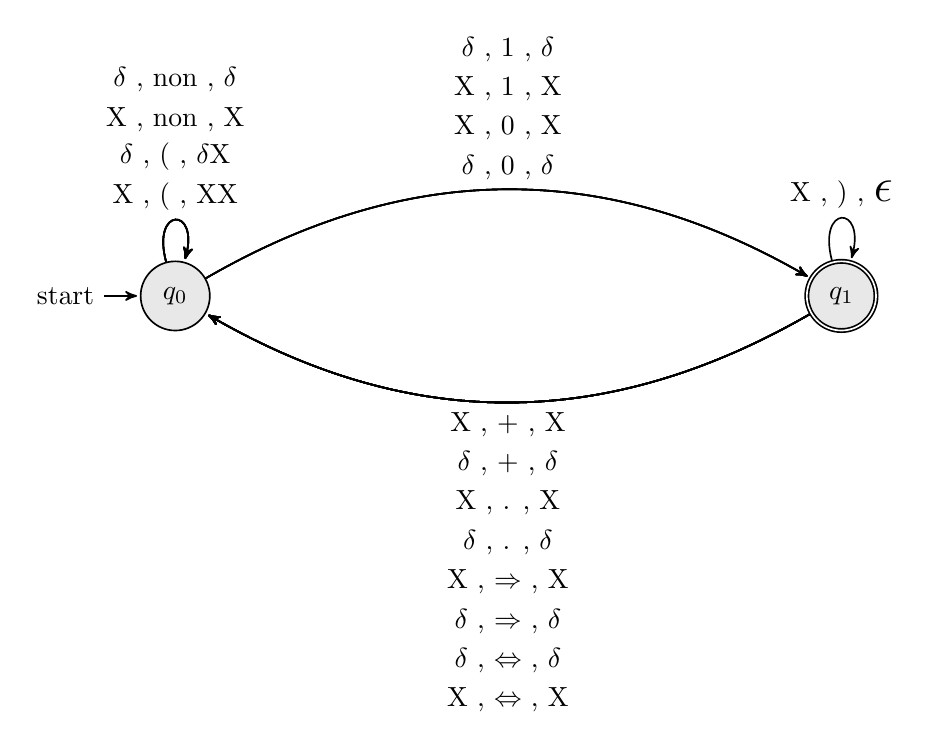
\begin{tikzpicture}[->,>=stealth',shorten >=1pt,auto,node distance=2.8cm,semithick]
  \tikzstyle{every state}=[fill={rgb:black,1;white,10}]

  \node[initial,state] 			(A)				{$q_0$};
  \node[state,accepting]         	(B) [right=8cm]	{$q_1$};

  \path		(A) 	edge	[loop above] 	node [above=1.5cm] {$\delta$ , non , $\delta$} (A)
  		(A)     edge	[loop above]	node [above=1cm]   {X , non , X} (A)
		(A)	edge	[loop above]	node [above=0.5cm] {$\delta$ , ( , $\delta$X} (A)
		(A)	edge	[loop above]	node {X , ( , XX} (A)
		
		(B)	edge	[loop above]	node{X , ) , \LARGE{$\epsilon$}} (B)

		(A) 	edge	[bend left]	node [above=1.5cm] {$\delta$ , 1 , $\delta$} (B)
		(A)	edge	[bend left]	node [above=1cm] {X , 1 , X} (B)
		(A) 	edge	[bend left] 	node [above=0.5cm] {X , 0 , X} (B)
		(A)	edge	[bend left]	node {$\delta$ , 0 , $\delta$} (B)

		(B)	edge	[bend left]	node {X  , + , X} (A)
		(B) 	edge	[bend left]	node [below=0.5cm] {$\delta$ , + , $\delta$} (A)
		(B) 	edge 	[bend left]	node [below=1cm] {X , . , X} (A)
		(B) 	edge 	[bend left] 	node [below=1.5cm] {$\delta$ , . , $\delta$} (A)
		(B)	edge	[bend left]	node [below=2cm] {X , $\Rightarrow$ , X} (A)
		(B)	edge	[bend left]	node [below=2.5cm] {$\delta$ , $\Rightarrow$ , $\delta$} (A)
		(B)	edge	[bend left]     node [below=3cm] {$\delta$ , $\Leftrightarrow$ , $\delta$} (A)
		(B)	edge	[bend left]	node [below=3.5cm] {X , $\Leftrightarrow$ , X} (A);
\end{tikzpicture}
\caption{Automate à pile qui reconnaît le language par état final et par pile vide.}
\end{center}
\end{figure}
\section*{Question 3}
\textit{
\textcolor{blue}{
\underline{Question:}
 Écrire une fonction en langage C qui teste si une liste de token appartient au langage ou non.
}
}
\newline\newline
Pour cette partie là du projet nous avons fait la fonction \textit{$recognize\_language(liste\_token A)$} qui va renvoyer 'true' si le l'expression utilisé par l'utilisateur est reconnu par l'automate et renvoie 'false' dans le cas contraire. Nous avons simulé les deux états q0 et q1 par un tableau T booléen qui contient les deux états, T[0] étant l'état inital et T[1] l'état final. Afin d'alléger le code source du projet, la pile qui empile ou dépile les parenthèses a été remplacé par un entier qui est incrémenté d'une unité lorsqu'on empile et est décrémenté d'une unité lorsqu'on dépile. La pile est donc vide lorsque sa valeur est de zéro. 
\newline
En fonction du type du 'token' on évolue ou pas d'un état à un autre. La boucle 'while' parcourt la liste des 'tokens' tant que celle-ci n'est pas vide. 'true' est renvoyé dans le cas où à la fin de la boucle 'while' l'état T[1] renvoie true et si la pile est vide (entier 'count' vaut zéro). Dans le cas contraire 'false' est renvoyé ce qui signifie que l'automate ne reconnaît pas l'expression utilisé par l'utilisateur.

\section*{Question 4}
\textit{
\textcolor{blue}{
\underline{Question:}
À partir de la liste de tokens et en utilisant l’automate à pile, créer l’arbre représentant l’expression booléenne. Vous pouvez utiliser la fonction qui teste si la liste des tokens appartient au langage en la modifiant.
}
}
\newline
\newline
L'énoncé nous a laissé suggérer que l'utilisation d'une pile était nécessaire pour construire l'arbre représentant l'expression booléenne. Après de multiples recherches sur internet et plusieurs réflexions sur les exemples du projet, nous avons remarqué que l'expression booléenne écrite par exemple '1.(0+1)' est la description infixe du parcours de son arbre booléen. Nous avons ainsi pensé que transformé cette liste de 'tokens' écrite en infixe serait plus facile à la construction de son arbre si nous avons la description de l'expression booléenne écrite en parcours suffixe. Pour cela nous avons utilisé la fonction \textit{$infix\_to\_postfix(liste\_token actual)$} qui va prendre en argument la liste de tokens entré par l'utilisateur \textit{(liste en parcours infixe de l'arbre correspondant)} et va renvoyé une liste de token en parcours suffixe tout en tenant compte de l'ordre de priorité des parenthèses. 
\newline\newline
Pour cela nous avons utilisé l'algorithme suivant:
\newline\newline
\fbox{
\begin{minipage}{1\textwidth}
\textit{X étant notre liste de token initiale et Y la liste de token finale}
\newline
1- Poussez "(" sur la pile et ajoutez ")" à la fin de X.\newline
2- Scannez X de gauche à droite et répétez les étapes 3 à 6 pour chaque élément de X jusqu'à ce que la pile soit vide.\newline
3- Si un opérande est rencontré, ajoutez-le à Y.\newline
4- Si une parenthèse gauche est rencontrée, poussez-la sur Stack.\newline
5- Si un opérateur est rencontré, alors:\newline
        Dépilez de Stack et ajoutez à Y chaque opérateur.\newline
        Ajouter un opérateur à la pile.\newline
        [Fin de If]\newline
6- Si une parenthèse droite est rencontrée, alors:\newline
        Sautez à plusieurs reprises de Stack et ajoutez à Y chaque opérateur (en haut de Stack) jusqu'à ce qu'une parenthèse gauche soit rencontrée.\newline
        Supprimez la parenthèse gauche.\newline
        [Fin de If]\newline
        [Fin de If]\newline
7- FIN.
\end{minipage}
}
\newline
\newline
Pour la suite nous avons eu besoin de la structure suivante qui nous permettra de construire l'arbre à partir de la liste de 'token':
\begin{verbatim}
struct noeud{
  struct noeud* sag;
  struct noeud* sad;
  type TYPE;
  union{
    bool value;             //if TYPE is a CONSTANT, value is 'true' if '1' else 'false' if '0'
    bool bracket;           //if TYPE is a BRACKET, value is 'true' if '(' else 'false' if ')'
    bool unary;             //if TYPE is a UNARY_OP, value is 'true' if 'NON' else 'false'
    op_binary OpBinary;     //if TYPE is a BINARY_OP, value depends on enum op_binary
  }attribute;
};
typedef struct noeud* arbre_token;
\end{verbatim}

Nous arrivons à la dernière étape de la réponse à cette question qui va consister à la construction de l'arbre à partir de notre liste de token trié préalablement dans l'ordre de lecture postfixe de l'arbre en tenant en compte la priorité des accordée aux parenthèses. 
\newline\newline
Pour cela nous avons utilisé l'algorithme suivant qui permet la construction de l'arbre:
\newline\newline
\fbox{
\begin{minipage}{1\textwidth}
\textit{X étant notre liste de token initiale}
\newline
1- Scannez X de gauche à droite et répétez les étapes 2 à 6 pour chaque élément de X jusqu'à ce que la pile soit vide.\newline
2- Transformez le token en un noeud Y.\newline
2- Si un opérande est rencontré, poussez-le sur Stack.\newline
	[FIN de If]\newline
3- Si un opérateur est rencontré, alors:\newline
	Dépilez Stack et ajoutez le noeud au fils droit de Y.\newline
	Dépilez Stack et ajoutez le noeud au fils gauche de Y.\newline
	[FIN de If]\newline
[FIn du scan]
4- Dépilez Stack et ajoutez le au noeud Y.\newline
5- Renvoyer Y.\newline
6- FIN.
\end{minipage}
}
\section*{Question 5}
\textit{
\textcolor{blue}{
\underline{Question:}
Calculer la valeur de l’expression arithmétique et afficher le résultat.
}
}
\end{document}
